\documentclass[12pt,a4paper]{article} 

\usepackage{fn2kursstyle}
\usepackage[russian]{babel}
\usepackage[T2A]{fontenc} 
\usepackage[utf8]{inputenc} 
\usepackage{geometry}
\usepackage{mathtools}
\usepackage{tikz}
\usepackage{pdfpages}
\usepackage[hidelinks]{hyperref}

\counterwithout{equation}{section}
\counterwithout{figure}{section}
\graphicspath{{pic/}}
\frenchspacing 

\newcommand{\picref}[1]{рис. \ref{#1}}
\newcommand{\half}{\frac{1}{2}}
\newcommand{\dhalf}{\dfrac{1}{2}}

\title{КУСОЧНО-ПАРАБОЛИЧЕСКИЙ МЕТОД НА ЛОКАЛЬНОМ ШАБЛОНЕ ДЛЯ ЗАДАЧ ГАЗОВОЙ ДИНАМИКИ}
\group{ФН2-62Б}
\author{А.\,И.~Токарев}
\supervisor{В.\,В.~Лукин}
\date{2022}

\begin{document}
    \maketitle
    \tableofcontents
    \pagebreak

    \section-{Введение}
    Одним из наиболее удачных вычислительных методов решения гиперболических уравнений является кусочно-параболический метод (с англ. Piecewise-Parabolic Method, PPM), разработанный для моделирования течения жидкостей и газов и применяемый в астрофизике. Он обладает порядком аппроксимации $ O(\tau^2 + h^3) $. Несмотря на великолепную точность, данный метод имеет ряд недостатков: концы парабол на разностных ячейках связываются путем реконструкции переменных на расширенном четырехточечном шаблоне, что повышает диссипацию в схеме. Кроме того, PPM дает достаточно точный результат на гадких решениях, а вот на разрывах происходят ощутимые осцилляции.

    Целью данной курсовой работы является анализ улучшенного метода PPM -- кусочно-параболический метод на локальном шаблоне (PPML). Его основное отличие заключается в том, что граничные точки парабол внутри разностых ячеек определяются с предыдущего временного слоя по методу характеристик, что позволяет точно описывать разрывные решения и избегать накопления лишней диссипации.
    
    В качестве анализа будет приведено сравнение точности методов PPM и PPML на примерах одномерных задач. Также проведем демонстрацию рассматриваемого метода на нескольких двумерных задач газовой динамики.

    \newpage
    
    \section{Постановка задачи}

    \subsection{Кусочно-параболический метод. PPM}
    Рассмотрим одномерную задачу. Пусть $\Omega_h$ -- множество узлов сетки, в общем случае неравномерной. Определим функцию $y(x)$ ее разностным аналогом $y_i, \, i = 1 \ldots n$ на этой сетке. Значения $y_i$ будем соотносить с центрами ячеек, а $ y_{ i + \half} = y_i^R $ и $ y_{i - \half} = y_i^L $ -- с концами. Строение разностной ячейки можно увидеть на \picref{fig:ppm_visual}

    \begin{figure}[h]
        \centering
        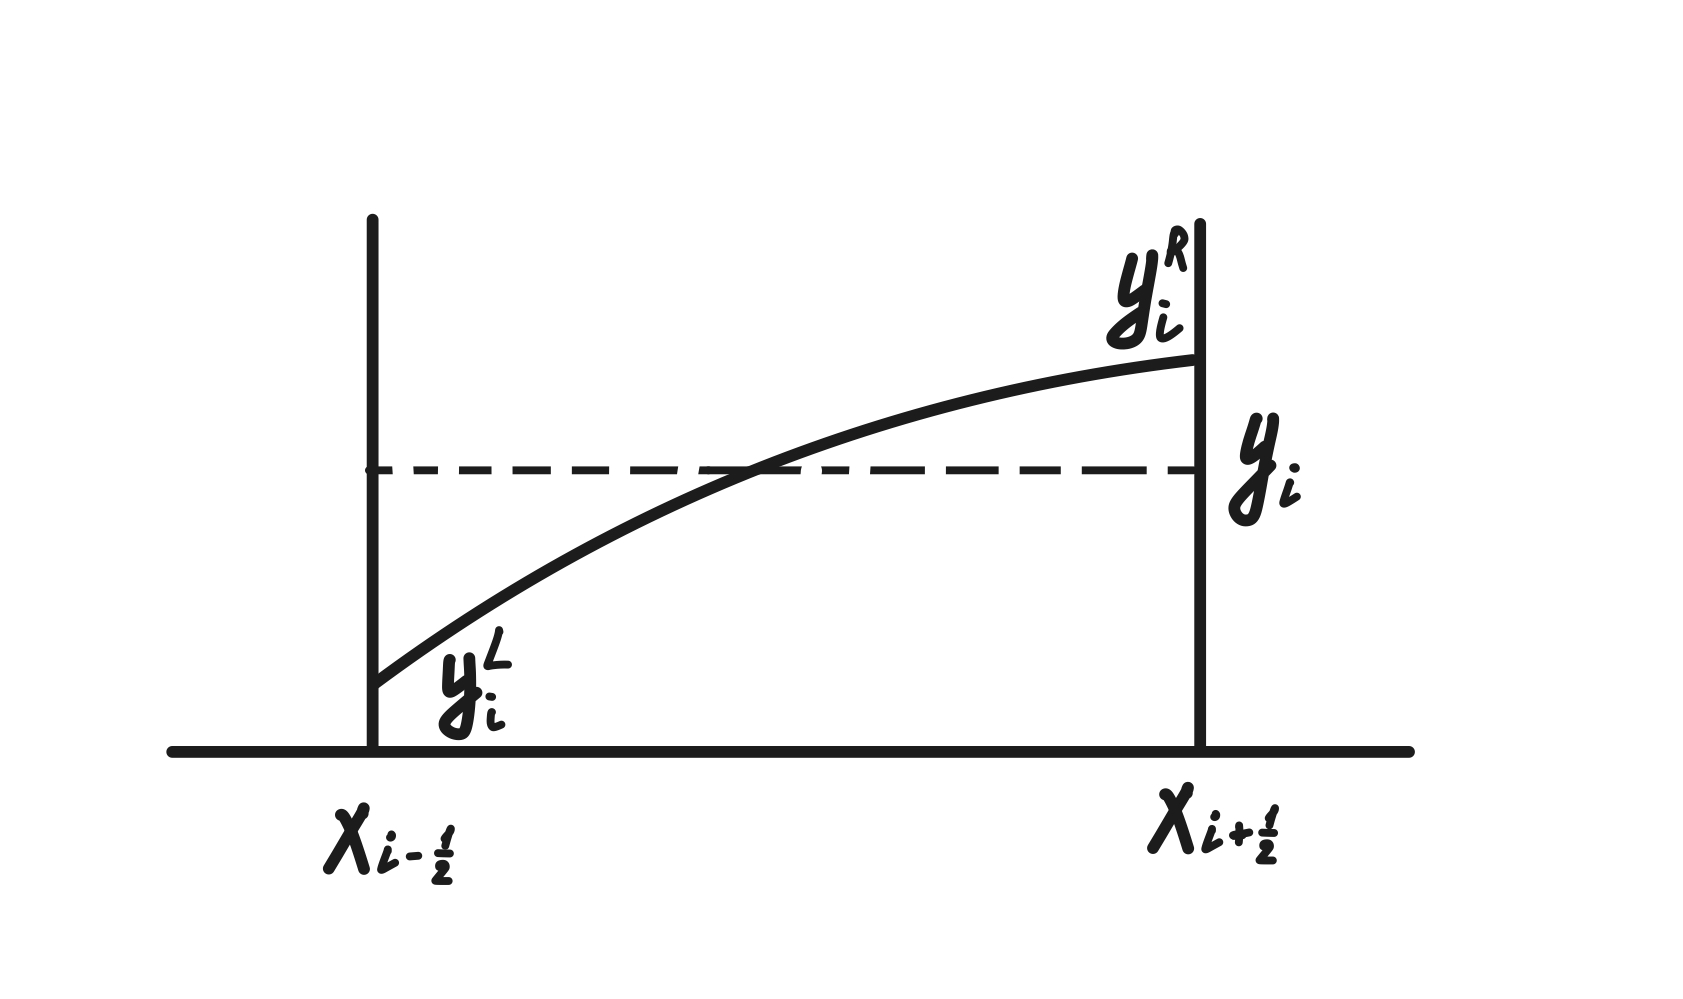
\includegraphics[width=0.5\textwidth]{ppm_visual.jpeg}
        \caption{Парабола внутри разностной ячейки}
        \label{fig:ppm_visual}
    \end{figure}

    Основная идея метода PPM заключается в следующем -- внутри отрезка $ [x_{i-\half}, x_{i+\half}] $ функцию $ y = y(x) $ можно аппроксимировать параболой:
    \begin{multline}
        \label{parabolic_eq}
        y(x) = y_i^L + \xi(\Delta y_i + y_i^{(6)}(1 - \xi)), \\
        \xi = (x - x_{i-\half})h^{-1}, \quad \Delta y_i = y_i^R-y_i^L, \quad y_i^{(6)} = 6\Bigl[ y_i - \half(y_i^R + y_i^L)\Bigr].
    \end{multline}

    Выражение \eqref{parabolic_eq} является квадратурной формулой для соотнешния:
    \[
        y(x_i) = \dfrac{1}{h} \displaystyle \int_{x_{i-\half}}^{x_{i+\half}} y(\chi) d\chi.
    \]

   Значение функции $ y(x) $ на границах при условиях гладкости и отсутствия экстремумов принадлежит отрезкам:
   \begin{equation}
        \label{boundary_nodes}
        y_{i-\half} \in [y_{i-1}, y_i], \qquad y_{i+\half} \in [y_i, y_{i+1}], 
   \end{equation}
   \noindent что дает возможность установить соответствие граничных узлов на соседних ячейках:
   \[
        \begin{split}
            y_i^R &= y_{i+1}^L = y_{i+\half} = \dhalf(y_i + y_{i+1}) - \dfrac{1}{6}(\delta y_{i+1} - \delta y_i), \\[0.7em]
            y_i^L &= y_{i-1}^R = y_{i-\half} = \dhalf(y_i + y_{i-1}) - \dfrac{1}{6}(\delta y_{i} - \delta y_{i-1}), 
        \end{split}
   \] 
   \noindent где 
   \[
        \delta y_i = \dhalf(y_{i+1} + y_{i-1}).
   \]

    Эта интерполяционная процедура имеет четвертый порядок. Чтобы обеспечить монотонность решения и выполнить условие \eqref{boundary_nodes}, значения $ \delta y_i $ нужно заменить на 
    \[
        \delta_m y_i = 
        \begin{cases}
            \min(|y_i|,\, 2|y_i - y_{i-1}|,\, 2|y_{i+1} - y_i|)\cdot sign(\delta y_i), & (y_{i+1} - y_i)(y_i - y_{i-1}) > 0, \\
            0, \quad (y_{i+1} - y_i)(y_i - y_{i-1}) \leq 0.
        \end{cases}  
    \]

    В областях немонотонного решения $ y(x) $ следует переопределять значения на границах, то есть $ y_i^L,\, y_i^R $. При этом возможны два сценария:
    \begin{itemize}
        \item $ y_i $ является локальным экстремумом, тогда на всем отрезке $ [x_{i-\half}, x_{i+\half}] $ функция $ y(x) = \text{const} $, а значит $ y_i^L = y_i^R = y_i $.
        
        \item $ y_i $ лежит слишком близко к границе, а при условии $|\Delta y_i| < | y_i^{(6)} |$ парабола может иметь экстремум внутри разностной ячейки. В этом случае $ y_i^L $ и $ y_i^R $ должны быть выбраны так, чтобы сдвинуть его к границам:
        \[
            \begin{split}
                y_i^L = 3y_i -2y_i^R, &\quad \Delta y_i \cdot y_i^{(6)} > (\Delta y_i)^2, \\
                y_i^R = 3y_i -2y_i^L, &\quad \Delta y_i \cdot y_i^{(6)} < -(\Delta y_i)^2.
            \end{split}  
        \]
    \end{itemize}

    После всех проделанных операция функцию $y(x)$ можно считать определенной на сетке $\Omega_h$. Рассмотрим среднее значение данной функции на отрезке $ [x_{i+\half-\alpha}, x_{i+\half}] $ (при $\alpha$ > 0):
    \[
        \overline y_{i+\half}^L(\alpha) = \dfrac{1}{\alpha} \displaystyle \int_{x_{i+\half-\alpha}}^{x_{i+\half}} y(x) dx = y_i^R - \dfrac{\alpha}{2h}\Bigl[ \Delta y_i - \Bigl( 1 - \dfrac{2 \alpha}{3h} \Bigr)y_i^{(6)} \Bigr].
    \]
    \begin{center}
        **** Линейное уравнение переноса и потоки ****
    \end{center}

    \subsection{Кусочно-параболический метод на локальном шаблоне. PPML}

    Интерполяционная процедура четвертого порядка, применяемая для переопределения граничных узлов, сглаживает разрывные решения $y(x)$. Чтобы обойти данное ограничение, можно определять $ y_i^L $ и $ y_i^R $ с помощью переноса значения на параболе с предыдущего шага по времени вдоль характеристики $ \frac{dx}{dt} = a $. Причем переопределять нужно лишь одну из границ. Для ясности впредь будем рассматривать $y_i^R = y_{i+\half}$.

    \section-{Заключение}

    \end{document}